%%%%%%%%%%%%%%%%%%%%%%%%%%%%%%%%%%%%%%%%%%%%%%%%%%%%%%%%%%%%%%%%%%%%%%%%%%%%%%%
\chapter{More basics}

%%%%%%%%%%%%%%%%%%%%%%%%%%%%%%%%%%%%%%%%%%%%%%%%%%%%%%%%%%%%%%%%%%%%%%%%%%%%%%%
\section{Choice of $\log$ / Determination $\tilde\theta$ of $\theta$}
\begin{figure}[!htbp] %{{{
  \centering
  \begin{subfigure}[b]{0.4\textwidth}
    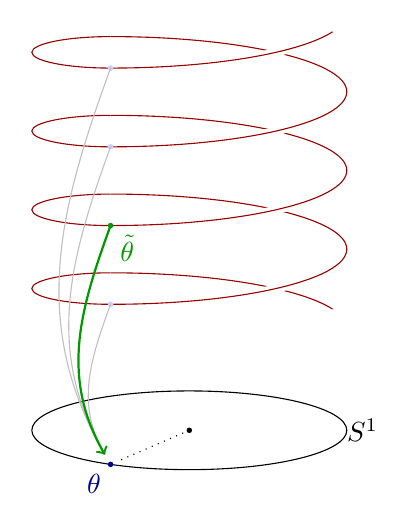
\begin{tikzpicture}[scale=1]
      \node[] (zero) at (0,0) {};
      \fill (zero) circle (1pt);
      \draw (0,-0.5) arc (270:-90:2 and 0.5);

      \node (theta) at ({cos(240) * 2},{sin(240) * 0.5}) {};
      % \node [below left of=theta,blue!40!white] {$\theta$};

      \draw[dotted] (0,0) -- (theta);
      \fill[blue!60!black] (theta) circle (1pt);


      \draw[red!60!black] (-1,2) arc (270:200:-3 and -0.7);
      \draw[line width=3pt,white] (-1,2) arc (270:90:1 and -0.2) arc (270:90:-3 and 0.7);
      \draw[red!60!black] (-1,2) arc (270:90:1 and -0.2) arc (270:90:-3 and 0.7);
      \fill[blue!20!white] (-1,1.6) circle (1pt);

      \draw[line width=3pt,white] (-1,3) arc (270:90:1 and -0.2) arc (270:90:-3 and 0.7);
      \draw[red!60!black] (-1,3) arc (270:90:1 and -0.2) arc (270:90:-3 and 0.7);
      \fill[green!60!black] (-1,2.6) circle (1pt);

      \draw[line width=3pt,white] (-1,4) arc (270:90:1 and -0.2) arc (270:90:-3 and 0.7);
      \draw[red!60!black] (-1,4) arc (270:90:1 and -0.2) arc (270:90:-3 and 0.7);
      \fill[blue!20!white] (-1,3.6) circle (1pt);

      \draw[line width=3pt,white] (-1,5) arc (270:90:1 and -0.2) arc (270:200:-3 and 0.7);
      \draw[red!60!black] (-1,5) arc (270:90:1 and -0.2) arc (270:200:-3 and 0.7);
      \fill[blue!20!white] (-1,4.6) circle (1pt);


      \draw[->,gray!50!white] (-1,1.6) to[out=250,in=120] (theta);
      \draw[->,gray!50!white] (-1,3.6) to[out=250,in=120] (theta);
      \draw[->,gray!50!white] (-1,4.6) to[out=250,in=120] (theta);
      \draw[->,green!60!black,thick] (-1,2.6) to[out=250,in=120] (theta);
      \node[below left,blue!60!black] at (theta) {$\theta$};
      \node[below right,green!60!black] at (-1,2.6) {$\tilde\theta$};

      \node[red!60!black] at (2.2,4.8) {$\R$};
      \node at (2.2,0) {$S^1$};
    \end{tikzpicture}
    \caption{Universal cover}
    \label{fig:univCover}
  \end{subfigure}%
  \qquad
  \begin{subfigure}[b]{0.4\textwidth}
    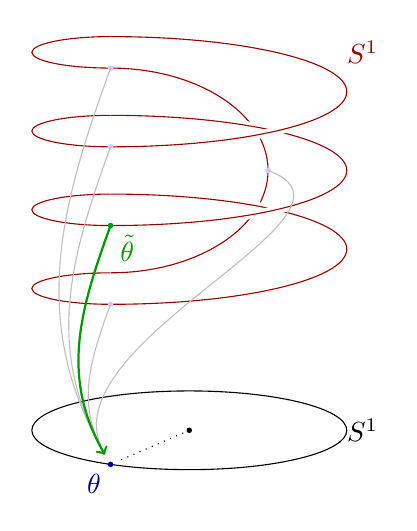
\begin{tikzpicture}[scale=1]
      \node[] (zero) at (0,0) {};
      \fill (zero) circle (1pt);
      \draw (0,-0.5) arc (270:-90:2 and 0.5);

      \node (theta) at ({cos(240) * 2},{sin(240) * 0.5}) {};
      % \node [below left of=theta,blue!40!white] {$\theta$};

      \draw[dotted] (0,0) -- (theta);
      \fill[blue!60!black] (theta) circle (1pt);


      \draw[line width=3pt,white] (-1,5) arc (270:90:1 and -0.2) arc (270:200:-3 and 0.7);
      \draw[red!60!black] (-1,5) arc (270:90:1 and -0.2) arc (270:90:-2 and -1.3);
      \fill[blue!20!white] (-1,4.6) circle (1pt);
      \fill[blue!20!white] (1,3.3) circle (1pt);

      % \draw[red!60!black] (-1,2) arc (270:200:-3 and -0.7);
      \draw[line width=3pt,white] (-1,2) arc (270:90:1 and -0.2) arc (270:90:-3 and 0.7);
      \draw[red!60!black] (-1,2) arc (270:90:1 and -0.2) arc (270:90:-3 and 0.7);
      \fill[blue!20!white] (-1,1.6) circle (1pt);

      \draw[line width=3pt,white] (-1,3) arc (270:90:1 and -0.2) arc (270:90:-3 and 0.7);
      \draw[red!60!black] (-1,3) arc (270:90:1 and -0.2) arc (270:90:-3 and 0.7);
      \fill[green!60!black] (-1,2.6) circle (1pt);

      \draw[line width=3pt,white] (-1,4) arc (270:90:1 and -0.2) arc (270:90:-3 and 0.7);
      \draw[red!60!black] (-1,4) arc (270:90:1 and -0.2) arc (270:90:-3 and 0.7);
      \fill[blue!20!white] (-1,3.6) circle (1pt);
   


      \draw[->,gray!50!white] (-1,1.6) to[out=250,in=120] (theta);
      \draw[->,gray!50!white] (-1,3.6) to[out=250,in=120] (theta);
      \draw[->,gray!50!white] (-1,4.6) to[out=250,in=120] (theta);
      \draw[->,gray!50!white] (1,3.3) to[out=-20,in=120] (theta);
      \draw[->,green!60!black,thick] (-1,2.6) to[out=250,in=120] (theta);
      \node[below left,blue!60!black] at (theta) {$\theta$};
      \node[below right,green!60!black] at (-1,2.6) {$\tilde\theta$};

      \node[red!60!black] at (2.2,4.8) {$S^1$};
      \node at (2.2,0) {$S^1$};
    \end{tikzpicture}
    \caption{$q$-sheet cover}
    \label{fig:qCover}
  \end{subfigure}
  \caption{Covers}\label{fig:covers}
\end{figure} %}}}
\paragraph{Universal cover:}
\[
  \R\to S^1; \nu \mapsto e^{i\nu}
\]
\TODO{}

\paragraph{$q$-sheet cover:}
\[
  S^1\to S^1; \nu \mapsto \nu^q
\]
\TODO{}

\paragraph{Multivalued functions:}
\begin{defn}
  \marginnote{\cite[227]{Balser2000Formal}}
  A function $f$, \rewrite{defined on some domain $G$ considered on the Riemann
  surface}, is called to be \emph{single-valued} if
  \[
    f(t)=f(t\exp(2\pi i)) \qquad\text{whenever both sides are defined.}
  \]
  \begin{s-rem}
    \begin{itemize}
      \item This is nothing else but saying that we may consider the function
        on the projection to the plane.
      \item The condition might be nowhere defined.
    \end{itemize}
  \end{s-rem}
  \begin{s-exmp}
    The function $t\to t^\alpha$ is single-valued whenever $\alpha\in\Z$.
  \end{s-exmp}
\end{defn}
\TODO{}

\paragraph{determination of a function:}
\TODO[principal determination of $x^{1/2}$]

%%%%%%%%%%%%%%%%%%%%%%%%%%%%%%%%%%%%%%%%%%%%%%%%%%%%%%%%%%%%%%%%%%%%%%%%%%%%%%%
\section{Čech cohomology}

%%%%%%%%%%%%%%%%%%%%%%%%%%%%%%%%%%%%%%%%%%%%%%%%%%%%%%%%%%%%%%%%%%%%%%%%%%%%%%%
\section{Semidirect products}
\begin{comment}
  see
  \begin{itemize}
    \item \url{http://nlab.mathforge.org/nlab/show/semidirect+product+group}
    \item \url{http://en.wikipedia.org/wiki/Semidirect_product}
    \item \cite{Robinson2003An}
  \end{itemize}
\end{comment}
We will refer to \cite[75]{Robinson2003An} for semidirect products.
Let $G$ be a group with a normal subgroup $N$ ($N\vartriangleleft G$) and a
subgroup $H$ such that 
\[
  G=NH\qquad\text{and}\qquad N\cap H=1.
\]
Then $G$ is said to be the \emph{(internal) semidirect product} of $N$ and $H$,
$G=N\rtimes H$.
\begin{rem}
  \begin{enumerate}
    \item Each element $g\in G$ has a unique decomposition $g=nh$ with $n\in N$
      and $h\in H$. Since
      \begin{itemize}
        \item[] for $g=n'h'$ another such expression, then
          $(n')^{-1}n=h'h^{-1}\in N\cap H=1$ such that $n=n'$ and $h=h'$.
      \end{itemize}
    \item Conjugation in $N$ by an element $h\in H$ defines an automorphism of
      $N$, say $\rho(h)$ which satisfies for $h_i\in H$
      \[
        \rho(h_1,h_2)=\rho(h_1)\rho(h_2)
      \]
      and thus $\rho:H\to\Aut(N)$ is a homomorphism.
  \end{enumerate}
\end{rem}
In the other direction, one can get from $N$, $H$ and a given homomorphism 
$\rho:H\to\Aut(N)$ the same structure back. This will be the so-called
\emph{external semidirect product}. It is defined by the underlying group
\[
  G:=\left\{(n,h)\mid n\in N,h\in H\right\}
\]
together with the multiplication
\begin{align*}
  G\times G&\to G
\\\left((n_1,h_1),(n_2,h_2)\right)&\mapsto(n_1\rho(h_1)(n_2),h_1h_2)
\end{align*}
with the identity element $(1_N,1_H)$ and the inverse of $(n,h)$ given by
$(\rho(h^{-1})(n^-1),h^-1)$. In $G$ there are the natural subgroups
\[
  \bar N=\{(n,1_H)\mid n\in N)\}
  \qquad\text{and}\qquad
  \bar H=\{(1_N,h)\mid h\in H)\}
\]
which are canonically isomorphic to $N$ and $H$ respectively. For $n\in N$ and
$h\in H$ we have
\[
  (n,1_H)(1_N,h)=(n\underset{\id_N}{\underbrace{\rho(1_H)}}(1_N),h)
  =(n,h)\in \bar N\bar H \,.
\]
It follows that $G=\bar N\bar H$ and $\bar N\cap\bar H=1$. To check that
$G=\bar N\rtimes\bar H$ we only have to show that $\bar N$ is normal in $G$.
Let $n,n'\in N$ and $h\in H$ then
\begin{align*}
  (n,h)(n',1_H)(n,h)^{-1}
  &=(n,h)(n',1_H)(\rho(h^{-1})(n^{-1}),h^{-1})
  \\&=(n\rho(h)(n'),h)(\rho(h^{-1})(n^{-1}),h^{-1})
  \\&=(n\rho(h)(n')\rho(h)\rho(h^{-1})(n^{-1}),1_H)
  \\&=(n\rho(h)(n')n^{-1},1_H) \in \bar N \,.
\end{align*}

In the case, where $\rho$ is the trivial homomorphism
\begin{align*}
  \rho:H&\to\Aut(N)
\\h&\mapsto \id_N
\end{align*}
the elements of $\bar N$ and $\bar H$ commute, so that $G$ becomes the direct
product $N\times H$. Thus the semidirect product is a generalization of the
direct product of two groups.

\TODO[from splitting exact sequence]

%%%%%%%%%%%%%%%%%%%%%%%%%%%%%%%%%%%%%%%%%%%%%%%%%%%%%%%%%%%%%%%%%%%%%%%%%%%%%%%
\section{Faithful representations} \label{sec:faithRepre}
\cite[Def.4.1]{hall2003lie} says the following about faithful representations:
\begin{defn}
  \begin{comment}
    See:
    \begin{itemize}
      \item \cite[Def.4.1]{hall2003lie}
      \item \url{http://nlab.mathforge.org/nlab/show/faithful+representation}
    \end{itemize}
  \end{comment}
  Let $G$ be a matrix\TODO[??] Lie group. Then a \emph{(finite-dimensional
  complex) representation} of $G$ is a Lie group homomorphism
  \[
    \rho:G\to\Gl(V)
  \]
  where
  \begin{itemize}
    \item $V$ is a finite-dimensional complex vector space.
  \end{itemize}
  If $\rho$ is a one-to-one homomorphism, then the representation is called
  \emph{faithful}.
  \begin{comment}
    \textbf{Other criterion:}
    If the associated homomorphism $G\to\Aut(V)$ is injective, then the
    representation is \emph{faithful}.
  \end{comment}
  \begin{s-rem}
    If a representation $\rho$ is a faithful representation of a matrix Lie
    group $G$ then $\{\rho(A)\mid A\in G\}$ is a group of matrices that is
    isomorphic to the original group $G$. Thus, $\rho$ allows us to represent
    $G$ as a group of matrices.
  \end{s-rem}
\end{defn}
